\documentclass[aspectratio=169]{beamer}
\usetheme{Madrid}
\usepackage[utf8]{inputenc}
\usepackage[T1]{fontenc}
\usepackage{tikz}
\usepackage{amssymb}
\usepackage{graphicx}
\setbeamertemplate{navigation symbols}{}
\setbeamercolor{title}{fg=white,bg=violet!70!purple}
\setbeamercolor{frametitle}{fg=white,bg=violet!70!purple}
\setbeamercolor{block title}{bg=violet!70!purple!20,fg=black}
\setbeamercolor{block body}{bg=violet!70!purple!8,fg=black}
\setbeamercolor{item}{fg=violet!70!purple}
\setbeamercolor{itemize item}{fg=violet!70!purple}
\setbeamertemplate{itemize item}[triangle]

\title{Story Studio 2 — Style It}
\subtitle{Background, heading colour, alignment, font size — CSS for your page}
\author{ByteForge --- Grade 7 --- Game Maker}
\date{}

\begin{document}

\begin{frame}
    \titlepage
\end{frame}

\begin{frame}{Today's Plan}
    \begin{itemize}
        \item Paint the Page
        \item Title Colour
        \item Center Stage
        \item Readable Text
        \item[$\bigstar$] BOSS --- Style the Front Page
    \end{itemize}
\end{frame}

\begin{frame}{Content vs. style — two different jobs}
    \large
    \begin{itemize}
        \item Last week's blocks decided WHAT is on the page. This week's Style blocks decide how it LOOKS
        \item Colours, alignment, size.
        \item Worked example: the exact same "My Story" heading, styled two ways — plain black text, or bold cyan text — is still 100\% the same HTML content. Only the CSS rule changed.
    \end{itemize}

    \begin{center}
    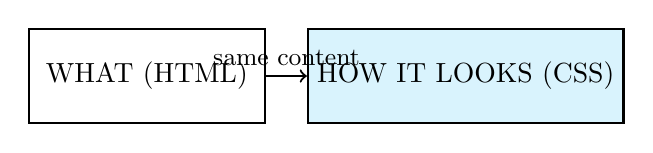
\begin{tikzpicture}[scale=0.9]

        \node[draw, thick, minimum width=3cm, minimum height=1.2cm] (a) at (0,0) {WHAT (HTML)};
        \node[draw, thick, fill=cyan!15, minimum width=3cm, minimum height=1.2cm] (b) at (4.5,0) {HOW IT LOOKS (CSS)};
        \draw[->, thick] (a) -- (b) node[midway, above] {\small same content};
    \end{tikzpicture}
    \end{center}
\end{frame}


\begin{frame}{A style rule can target ONE kind of block}
    \large
    \begin{itemize}
        \item "Set heading colour" only changes headings
        \item Paragraphs stay whatever colour they already were. A targeted rule, not a blanket one.
    \end{itemize}
\end{frame}


\begin{frame}{Alignment is a choice, not a colour}
    \large
    \begin{itemize}
        \item Unlike colour, alignment only has a few real choices
        \item Left, center, right. Centered paragraphs are actually harder to read line-by-line.
    \end{itemize}
\end{frame}


\begin{frame}{Font size affects real readability}
    \large
    \begin{itemize}
        \item Text that's too small is a genuine accessibility problem
        \item Real design guidelines set a minimum readable size (commonly 16px).
        \item Worked example: print "Hello" at 10px and at 24px side by side (or just hold up two phones at different zoom levels) — ask which one someone with poor eyesight could actually read across a room.
    \end{itemize}
\end{frame}


\begin{frame}{BOSS — HTML gives structure, CSS gives style}
    \large
    \begin{itemize}
        \item Unlike HTML tags, CSS rules apply no matter when you set them
        \item Style first or last, the result is identical.
    \end{itemize}
\end{frame}

\begin{frame}{Real-World Examples}
    \large
    \begin{itemize}
        \item Toggle a phone's font size / "reader mode" setting live, or compare a site with tiny 10px body text against one with proper 16px+ text
        \item Ask which one people would actually keep reading. Minecraft's own "resource packs" are exactly this idea at game-scale: the SAME blocks and items (the content), completely re-skinned to look different (the style).
    \end{itemize}
\end{frame}


\begin{frame}{Image}
    \begin{center}
    
\includegraphics[width=0.5\textwidth]{images/css.png}

    \large The real language behind every Style block you just used.

    \small CSS logo — W3C, public domain, via Wikimedia Commons
    \end{center}
\end{frame}

\begin{frame}{Let Them Discover}
    \Large
    Find one website that centers a whole paragraph of body text (not a title). Read it aloud line by line — does the centering make it harder to follow? Why do titles get away with it but paragraphs don't?
\end{frame}

\begin{frame}{Your Turn}
    \Large
    Open the student map, find \textbf{Story Studio 2 — Style It}, and work through it
    hands-on --- everything you just saw, they now do themselves.
\end{frame}

\end{document}
